%% ==============================================================================
%% content/05-resultats.tex
%% Chapitre 5 : Bibliographie Programmable et Compilation Automatisée (biblio/ & latexmkrc)
%% ==============================================================================
\chapter{Bibliographie Programmable et Compilation Automatisée}
\label{chap:biblio-compilation}

\section{La Révolution Bib\LaTeX{} et Biber}
\label{sec:biblatex-biber}

Pendant plusieurs décennies, la gestion des références bibliographiques reposait sur le moteur historique \code{BibTeX}.
Bien qu'extrêmement robuste, \code{BibTeX} présentait des limites rédhibitoires pour les auteurs contemporains :
\begin{itemize}
  \item les styles étaient programmés dans un langage obscur de type Forth (les fichiers \code{.bst}),
  \item la prise en charge des caractères accentués et de l'encodage UTF-8 était défaillante,
  \item et toute modification de ponctuation ou d'ordre des auteurs nécessitait un savoir-faire d'initié.
\end{itemize}

Comme le documentent \textcite{lehman2024biblatex}, Bib\LaTeX{}, adossé au moteur de tri moderne \code{Biber},
a profondément rénové cette discipline.
En transférant la logique de mise en forme directement dans le langage \LaTeX{},
Bib\LaTeX{} permet de concevoir des styles entièrement programmables et modulaires.

Dans notre projet, cette couche est externalisée dans le dossier \code{biblio/}
à travers trois fichiers complémentaires :
\begin{enumerate}
  \item \textbf{\code{references.bib} :} la base de données brute des notices (auteurs, titres, dates, DOI, URL).
  \item \textbf{\code{custom-style.bbx} :} la mise en page de la bibliographie finale imprimée en fin d'ouvrage.
  \item \textbf{\code{custom-style.cbx} :} la mise en page des renvois et des citations dans le cours du texte.
\end{enumerate}

\section{Personnalisation de la Bibliographie Finale : \code{custom-style.bbx}}
\label{sec:bbx-detail}

Le fichier \code{custom-style.bbx} hérite de la classe de référence \code{authoryear}
et applique plusieurs raffinements typographiques :

\begin{itemize}
  \item \textbf{Noms en petites capitales :}
  grâce à la macro \code{\textbackslash mkbibnamefamily},
  les noms de famille apparaissent en petites capitales (\textsc{Majuscules Réduites}) sans alourdir le texte.
  \item \textbf{Distinction visuelle des titres :}
  les titres d'articles ou d'actes de conférences sont placés entre guillemets de langue active (\code{\textbackslash enquote}),
  tandis que les titres d'ouvrages et de thèses sont composés en italique (\code{\textbackslash mkbibemph}).
  \item \textbf{Hyperliens d'identifiants DOI et URL :}
  les identifiants numériques sont formatés sous forme de liens compacts cliquables
  (par exemple \code{doi:10.1016/...}) renvoyant directement vers la publication originale de l'éditeur.
  \item \textbf{Espacement vertical maîtrisé :}
  le paramètre \code{\textbackslash bibitemsep} ajuste le blanc typographique entre deux notices successives.
\end{itemize}

\section{L'Art de Citer dans le Texte : \code{custom-style.cbx}}
\label{sec:cbx-detail}

Dans le corps de texte, le fichier \code{custom-style.cbx} gouverne la façon dont les renvois apparaissent :

\begin{itemize}
  \item \textbf{Citation parentétique (\code{\textbackslash autocite} ou \code{\textbackslash parencite}) :}
  à privilégier pour étayer une affirmation scientifique sans interrompre la lecture courante.
  Exemple : \autocite{knuth1984texbook}.
  \item \textbf{Citation intégrée au discours (\code{\textbackslash textcite}) :}
  à utiliser lorsque l'auteur fait partie intégrante de la phrase grammaticale.
  Exemple : \textcite{lamport1994latex} a développé le premier macro-système \LaTeX{}.
  \item \textbf{Gestion des co-auteurs :}
  le réglage \code{maxcitenames=2} assure que les articles ayant jusqu'à deux auteurs
  affichent les deux noms (ex. \textcite{mittelbach2023latex}),
  tandis qu'au-delà de deux auteurs,
  la formule « et al. » est insérée (ex. \textcite{lehman2024biblatex}).
  \item \textbf{Lien hypertexte intégral :}
  l'auteur et l'année sont cliquables, téléportant le lecteur directement sur la notice correspondante.
\end{itemize}

\section{Automatisation de la Compilation avec \code{latexmkrc}}
\label{sec:compilation-latexmkrc}

La compilation manuelle d'un document complet (comprenant la table des matières,
les renvois croisés et la bibliographie) requiert traditionnellement une longue suite de commandes :
\code{lualatex}, puis \code{biber}, puis à nouveau deux passes de \code{lualatex}.

Le fichier \code{latexmkrc} placé à la racine du projet automatise entièrement cette chorégraphie.
Il configure le programme \code{latexmk} avec les réglages optimaux :
\begin{itemize}
  \item \textbf{Moteur Lua\LaTeX{} par défaut :} paramétré via \code{\$pdf\_mode = 4;}.
  \item \textbf{Moteur Biber automatique :} paramétré via \code{\$bibtex\_use = 2;}.
  \item \textbf{Confinement dans le dossier \code{build/} :} paramétré via \code{\$out\_dir = 'build';}.
\end{itemize}

\begin{callout}[Avantage majeur du dossier build/]
Grâce au paramètre \code{\$out\_dir = 'build'}, les dizaines de fichiers temporaires générés par \LaTeX{}
(\code{.aux}, \code{.bbl}, \code{.bcf}, \code{.log}, \code{.toc}, \code{.synctex.gz})
ne polluent plus jamais la racine de votre projet !
La racine reste immaculée, claire et agréable à naviguer.
\end{callout}

Pour compiler l'intégralité du document en une seule touche, tapez simplement dans votre terminal :
\begin{center}
  \code{latexmk}
\end{center}
Le PDF compilé pour la lecture ou l'impression est généré dans le dossier \code{build/main.pdf}.
Pour faire le ménage et supprimer les fichiers temporaires, utilisez \code{latexmk -c} (nettoyage intermédiaire)
ou \code{latexmk -C} (nettoyage complet incluant le PDF).

\section{Traitement de Données et Visualisation avec Python (\code{uv})}
\label{sec:python-pipeline}

L'exploitation des données scientifiques en thèse repose sur une coopération étroite
entre les bibliothèques de calcul Python et le moteur de composition \LaTeX{}.
Pour garantir une reproductibilité stricte et éliminer les conflits de dépendances,
le projet s'appuie sur le gestionnaire moderne \code{uv} et son environnement virtuel dédié (\code{pyproject.toml}).

Le script d'orchestration \code{scripts/generate\_plots.py} s'exécute en une commande :
\begin{center}
  \code{uv run python scripts/generate\_plots.py}
\end{center}

Il matérialise deux flux d'ingénierie distincts selon la densité et la nature de vos représentations graphiques :

\subsection[Cas 1 : Données tabulaires compactes vers Tracé vectoriel natif]{Cas 1 : Données tabulaires compactes \texorpdfstring{$\to$}{vers} Tracé vectoriel natif \texorpdfstring{\code{pgfplots}}{pgfplots}}
\label{subsec:cas1-pgfplots}

Pour des courbes 2D (quelques dizaines à quelques centaines de points),
la méthode d'excellence consiste à exporter un fichier CSV compact dans \code{data/benchmark-results.csv}.
Le tracé est ensuite entièrement composé par le paquet \code{pgfplots} dans le manuscrit,
comme illustré sur le \cref{fig:courbe-csv} :

\begin{figure}[htbp]
  \centering
  \begin{tikzpicture}
    \begin{axis}[
      width=0.88\textwidth,
      height=6.2cm,
      grid=major,
      grid style={line width=0.4pt, draw=ThesisMuted!30},
      xlabel={Itérations d'entraînement},
      ylabel={Précision (\%)},
      xmin=1, xmax=20,
      ymin=50, ymax=102,
      legend pos=south east,
      legend cell align={left},
      legend style={
        draw=ThesisSecondary!35,
        line width=0.6pt,
        fill=white,
        fill opacity=0.92,
        text opacity=1,
        rounded corners=2pt,
        font=\footnotesize\sffamily,
        inner sep=4.5pt
      }
    ]
      \addplot[
        color=ThesisPrimary,
        line width=1.3pt,
        mark=*,
        mark size=1.8pt
      ] table[x=Iteration, y=AccuracyProposed, col sep=comma] {data/benchmark-results.csv};
      \addlegendentry{Architecture modulaire proposée}

      \addplot[
        color=ThesisAccent,
        line width=1.1pt,
        dashed,
        mark=square*,
        mark size=1.6pt
      ] table[x=Iteration, y=AccuracyBaseline, col sep=comma] {data/benchmark-results.csv};
      \addlegendentry{Modèle standard de référence}
    \end{axis}
  \end{tikzpicture}
  \caption[Courbes comparatives de précision générées depuis un CSV]{Convergence comparée de la précision (\%) générée en temps réel par \code{pgfplots} depuis \code{data/benchmark-results.csv}}
  \label{fig:courbe-csv}
\end{figure}

Comme visible sur le \cref{fig:courbe-csv}, les deux dynamiques partagent la même échelle verticale :
l'architecture proposée franchit le seuil des \SI{98}{\percent} dès la douzième itération,
tandis que le modèle de référence plafonne à \SI{83}{\percent}.
L'harmonie typographique est totale : les fontes, graisses et espacements sont rigoureusement identiques à ceux du corps de texte.

\subsection[Cas 2 : Graphique 2D haute résolution exporté par Matplotlib]{Cas 2 : Graphique 2D haute résolution exporté par Matplotlib}
\label{subsec:cas2-python2d}

Pour les représentations 2D complexes comportant des calculs d'intervalles de confiance,
des ajustements non linéaires ou de multiples séries temporelles,
l'export direct au format PDF vectoriel depuis Python constitue une alternative d'une grande fluidité.
Le script \code{scripts/generate\_plots.py} génère la figure \code{figures/python-benchmark.pdf}
dont l'intégration dans \LaTeX{} est immédiate (\cref{fig:python-benchmark}) :

\begin{figure}[htbp]
  \centering
  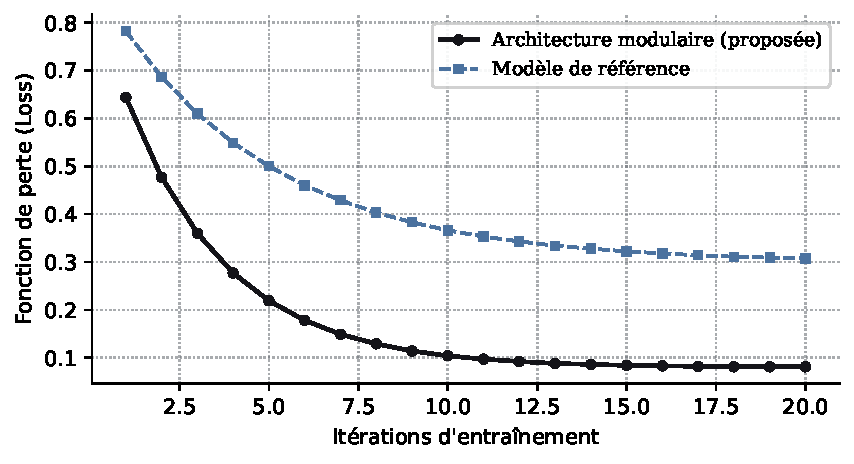
\includegraphics[width=0.82\textwidth]{figures/python-benchmark}
  \caption[Évolution des fonctions de perte générée par Python]{Convergence comparée des fonctions de perte (\textit{Loss}) générée en PDF vectoriel par Matplotlib via l'environnement \code{uv}}
  \label{fig:python-benchmark}
\end{figure}

Les étiquettes d'axes, les légendes et la palette chromatique sont calibrées pour s'accorder
rigoureusement avec la charte graphique de la thèse sans aucune pixellisation.

\subsection[Cas 3 : Visualisation 3D complexe vers Export vectoriel direct]{Cas 3 : Visualisation 3D complexe \texorpdfstring{$\to$}{vers} Export vectoriel direct via Python}
\label{subsec:cas3-python3d}

À l'inverse, dès qu'une figure met en jeu des représentations denses (surfaces tridimensionnelles,
cartes thermiques à forte résolution ou nuages de plus de \num{10000} points),
demander à \LaTeX{} d'en calculer le maillage provoque une saturation immédiate de la mémoire TeX
et multiplie le temps de compilation par dix.

Pour ces cas exigeants, le script Python pré-calcule la projection géométrique
et exporte directement une figure vectorielle dans \code{figures/python-3d-surface.pdf}.
Le document \LaTeX{} se contente de l'inclure instantanément via \code{\textbackslash includegraphics} (\cref{fig:surface-3d}) :

\begin{figure}[htbp]
  \centering
  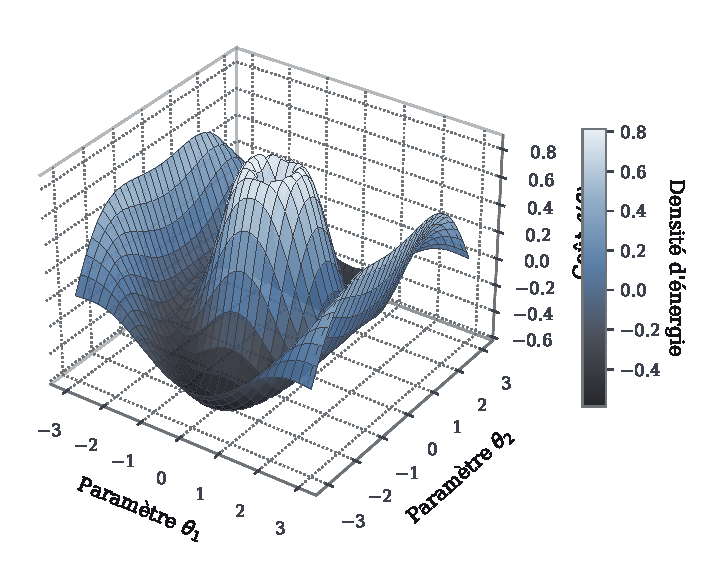
\includegraphics[width=0.84\textwidth]{figures/python-3d-surface}
  \caption[Paysage d'optimisation 3D généré par Python et \code{uv}]{Paysage de coût tridimensionnel non-convexe et trajectoire de descente générés par Matplotlib via l'environnement \code{uv} (\code{scripts/generate\_plots.py})}
  \label{fig:surface-3d}
\end{figure}

Pour garantir une harmonisation visuelle sans faille, le script Python respecte deux consignes strictes :
\begin{enumerate}
  \item \textbf{Échelle d'empagement calibrée :} les dimensions sont fixées par \code{figsize=(5.6, 3.8)} pouces,
  évitant tout redimensionnement qui altérerait la taille des étiquettes d'axes.
  \item \textbf{Palette chromatique coordonnée :} le dégradé de surface s'appuie sur les couleurs du document
  (\code{ThesisPrimary}, \code{ThesisSecondary} et \code{ThesisAccent}).
\end{enumerate}

\section{Interactivité PDF Avancée : les Calques OCG}
\label{sec:interactivite-ocg}

\subsection{Démystifier l'interactivité et compatibilité des visionneuses}
L'ajout de calques interactifs (\textit{Optional Content Groups} ou OCG, norme ISO 32000-1)
via le paquet \code{ocgx2} permet d'alléger un manuscrit en proposant des lectures à plusieurs niveaux.
Toutefois, son comportement dépend de la visionneuse PDF employée :

\begin{itemize}
  \item \textbf{Visionneuse intégrée VS Code / Navigateurs web (\code{pdf.js}) :}
  ces lecteurs légers n'implémentent pas les actions interactives sur les liens (\code{/SetOCGState}).
  Cliquer sur un bouton y reste inopérant par limitation du lecteur web.
  \item \textbf{Lecteurs PDF complets (Adobe Acrobat Reader, Foxit, PDF-XChange) :}
  les boutons de bascule fonctionnent immédiatement et permettent d'afficher ou masquer les couches en un clic.
  Les calques sont également pilotables depuis le panneau latéral « Calques » de l'application.
  \item \textbf{Version papier (\code{[print]}) :}
  les boutons interactifs sont totalement neutralisés à la compilation
  via les commandes de profil (\code{\textbackslash screenonly}),
  évitant tout élément orphelin ou inopérant sur le support physique.
\end{itemize}

\subsection[Cas d'usage : Encadré à bascule interactive]{Cas d'usage : Encadré à bascule interactive (Synthèse \texorpdfstring{$\longleftrightarrow$}{vs} Détails)}
L'encadré ci-dessous illustre une application professionnelle et sobre de cette technologie :
un bouton permet d'alterner entre une synthèse textuelle concise et le relevé exhaustif des données :

\begin{callout}[\ifprint{Synthèse et Métriques Détaillées à Convergence}{Encadré Interactif : Vue Synthétique vs Détails Métriques}]
  \screenonly{%
    \noindent
    \ocgbutton{ocg_box_syn ocg_box_det}{%
      Basculer la vue : Synthèse $\longleftrightarrow$ Métriques détaillées%
    }%
    \par\vspace{8pt}%
  }%
  \ocgstack{%
    \begin{ocg}{Vue Synthétique}{ocg_box_syn}{1}%
      \textbf{Comportement asymptotique de l'optimiseur :}\par\vspace{3pt}
      La convergence exponentielle observée sur l'architecture modulaire démontre que la décroissance de la perte suit la loi $\mathcal{L}(t) = \mathcal{L}_\infty + \alpha \mathrm{e}^{-\beta t}$.
      Le découplage structurel élimine les interférences de gradient et stabilise le conditionnement du système.
    \end{ocg}%
  }{%
    \begin{ocg}{Tableau Détaillé}{ocg_box_det}{0}%
      \textbf{Relevé comparatif des performances à convergence :}\par\vspace{3pt}
      \begin{tabularx}{\linewidth}{@{} >{\raggedright\arraybackslash}X r r r @{}}
        \toprule
        \textbf{Configuration} & \textbf{Précision finale} & \textbf{Perte résiduelle} & \textbf{Gain mesuré} \\
        \midrule
        Modèle de référence    & \SI{82.4}{\percent}       & 0.305                     & Référence \\
        Architecture proposée  & \SI{98.9}{\percent}       & 0.084                     & $+$\SI{16.5}{\percent} \\
        \bottomrule
      \end{tabularx}%
    \end{ocg}%
  }
\end{callout}

\subsubsection[Gestion intelligente Écran vs Impression]{Gestion intelligente Écran (\code{screen}) vs Impression Papier (\code{print})}
Le traitement des calques et des boutons interactifs met en lumière la puissance du découplage de classe :
\begin{itemize}
  \item \textbf{En profil numérique (\code{\textbackslash documentclass[screen]\{mythesis\}})} :
  le bouton interactif s'affiche et permet d'alterner dynamiquement entre la synthèse et le tableau, grâce à la superposition géométrique parfaite \code{\textbackslash ocgstack} pilotée par TikZ.
  \item \textbf{En profil imprimé (\code{\textbackslash documentclass[print]\{mythesis\}})} :
  \begin{enumerate}
    \item Les boutons interactifs (\code{\textbackslash ocgbutton}) sont \textbf{strictement omis} via \code{\textbackslash screenonly} : aucun bouton orphelin ou inopérant n'apparaît sur la feuille de papier.
    \item Les calques PDF (\code{ocg}) sont neutralisés pour supprimer tout objet OCG risquant de perturber les imprimantes professionnelles ou les RIP offset.
    \item La macro \code{\textbackslash ocgstack[both]\{...\}\{...\}} aplatit les deux contenus de manière séquentielle et aérée : le lecteur papier bénéficie ainsi à la fois du paragraphe de synthèse ET du tableau de données sans perte d'information.
    (Il est possible de ne conserver qu'une seule vue sur papier en spécifiant l'option \code{\textbackslash ocgstack[first]} ou \code{\textbackslash ocgstack[second]}).
  \end{enumerate}
\end{itemize}

\section{Outillage de Qualité Logicielle : \code{.editorconfig} et \code{.chktexrc}}
\label{sec:qualite-outils}

Pour pérenniser le travail d'équipe et garantir une hygiène rédactionnelle exemplaire,
le projet intègre deux fichiers de métaconfiguration indispensables :

\subsection{Standardisation de l'éditeur : \code{.editorconfig}}
Le fichier \code{.editorconfig} impose des conventions d'édition universelles reconnues par VS Code, Vim, Emacs et les pipelines \code{latexindent} :
\begin{itemize}
  \item Indentation stricte à 2 espaces pour l'ensemble des fichiers \LaTeX{} (\code{.tex}, \code{.cls}, \code{.sty}, \code{.clo}, \code{.bib}).
  \item Encodage UTF-8 et fins de ligne uniformisées en format Unix (\code{LF}).
  \item Suppression automatique des espaces superflues en fin de ligne lors de l'enregistrement.
\end{itemize}

\subsection{Linter typographique : \code{.chktexrc}}
Le linter \code{chktex} analyse le code source pour détecter les entorses aux règles de l'art typographique.
Le fichier \code{.chktexrc} fourni configure les règles métier :
\begin{itemize}
  \item \textbf{Obligation d'espaces insécables (\code{\textasciitilde}) :}
  il alerte immédiatement si un auteur oublie le tilde insécable avant un renvoi
  (ex. \code{\textbackslash cref\{...\}} ou \code{\textbackslash autocite\{...\}}),
  empêchant qu'une référence ou un numéro ne soit orphelin en début de ligne.
  \item \textbf{Filtrage des faux positifs :}
  il neutralise les alertes obsolètes pour les environnements de programmation modernes (\code{tcolorbox}, \code{listings}).
\end{itemize}

\section{Recette Pratique : Basculer entre Écran et Impression}
\label{sec:recette-bascule}

Le passage d'une version numérique interactive à une version papier prête pour l'imprimeur
ne demande **aucune modification** dans vos chapitres ou vos tableaux.
Ouvrez simplement le fichier maître \code{main.tex} et modifiez la toute première ligne :

\begin{itemize}
  \item \textbf{Pour la lecture sur écran :}
  \begin{center}
    \code{\textbackslash documentclass[screen]\{mythesis\}}
  \end{center}
  \item \textbf{Pour l'impression papier reliée :}
  \begin{center}
    \code{\textbackslash documentclass[print]\{mythesis\}}
  \end{center}
\end{itemize}
Relancez \code{latexmk} : votre document reconfigure instantanément sa pagination, ses marges,
son décalage de pliure \code{BCOR} et le traitement chromatique de ses liens hypertextes.
